%-------------------------------------------------------------------------------
%   CHAPTER 2 - RESEARCH
%-------------------------------------------------------------------------------

\section{Онолын болон харьцуулсан судалгаа}

\subsection{Онолын судалгаа}
Энэ хэсэгт B2B түгээлтийн бизнесийн процесс, логистик систем, маршрутын оновчлол, болон гар утасны хөгжүүлэлтийн технологиудын талаарх онолын ойлголтуудыг дэлгэрэнгүй авч үзнэ.

\subsubsection{Нийлүүлэлтийн сүлжээний удирдлага (SCM)}
Нийлүүлэлтийн сүлжээний удирдлага (Supply Chain Management - SCM) нь түүхий эд бэлтгэн нийлүүлэгчээс эхлээд эцсийн хэрэглэгч хүртэлх бараа, үйлчилгээ, мэдээлэл, санхүүгийн урсгалыг төлөвлөх, хэрэгжүүлэх, хянах цогц үйл ажиллагаа юм. Орчин үед SCM нь зөвхөн ложистик бус, мэдээллийн технологитой нягт уялдаж, "Ухаалаг нийлүүлэлтийн сүлжээ" (Smart Supply Chain) болон хөгжиж байна. SCM-ийн үндсэн зорилго нь нийлүүлэлтийн сүлжээний нийт зардлыг бууруулахын зэрэгцээ хэрэглэгчийн сэтгэл ханамжийг дээд зэргээр хангахад оршино.

\textbf{SCM-ийн үндсэн бүрэлдэхүүн хэсгүүд:}
\begin{itemize}
    \item \textbf{Төлөвлөлт (Planning):} Эрэлтийг таамаглах, нөөцийг төлөвлөх.
    \item \textbf{Худалдан авалт (Sourcing):} Нийлүүлэгчийг сонгох, гэрээ байгуулах.
    \item \textbf{Үйлдвэрлэл (Making):} Түүхий эдийг бэлэн бүтээгдэхүүн болгох.
    \item \textbf{Түгээлт (Delivering):} Логистик, агуулах, тээвэрлэлт.
    \item \textbf{Буцаалт (Returning):} Гэмтэлтэй эсвэл илүүдэл барааг буцаах үйл явц.
\end{itemize}

\subsubsection{B2B Түгээлтийн процесс ба онцлог}
B2B (Business-to-Business) түгээлт нь үйлдвэрлэгчээс бөөний худалдаачид, эсвэл бөөний худалдаачдаас жижиглэн худалдаачид руу бараа нийлүүлэх үйл явц юм. B2C (Business-to-Consumer) хүргэлтээс ялгаатай нь:
\begin{itemize}
    \item \textbf{Захиалгын хэмжээ:} B2B захиалга нь ихэвчлэн тоо хэмжээний хувьд их, овор хэмжээ томтой байдаг.
    \item \textbf{Давтамж:} Тогтмол хуваарийн дагуу, давтагдах шинж чанартай (жишээ нь: долоо хоног бүрийн Даваа гарагт).
    \item \textbf{Харилцаа:} Урт хугацааны гэрээт харилцаанд суурилдаг бөгөөд итгэлцэл чухал үүрэгтэй.
    \item \textbf{Шийдвэр гаргалт:} Олон шат дамжлагатай, оновчтой байдлыг чухалчилдаг. Худалдан авалтын шийдвэрийг сэтгэл хөдлөлөөр бус, үр ашгийн тооцооллоор гаргадаг.
\end{itemize}

\subsubsection{Last-Mile Delivery (Сүүлийн цэгийн хүргэлт)}
"Last-Mile Delivery" гэдэг нь барааг түгээлтийн төвөөс эцсийн хэрэглэгч (дэлгүүр эсвэл хувь хүн) хүртэл хүргэх логистикийн сүүлийн үе шатыг хэлнэ. Энэ нь нийлүүлэлтийн сүлжээний хамгийн өндөр зардалтай (нийт зардлын 53\% хүртэл), хамгийн их цаг хугацаа шаардсан, хамгийн төвөгтэй хэсэгт тооцогддог. Улаанбаатар хотын нөхцөлд замын түгжрэл, хаягжилтын асуудал нь Last-Mile Delivery-ийн үр ашгийг эрс бууруулдаг.

\subsubsection{Маршрутын оновчлол (Route Optimization)}
Хүргэлтийн зардлыг бууруулах, цаг хугацааг хэмнэхэд маршрутын оновчлол чухал үүрэгтэй. Энэ нь "Traveling Salesman Problem" (TSP) буюу олон цэгт хүргэлт хийх хамгийн дөт, үр ашигтай замыг тооцоолох математик аргачлал дээр суурилдаг. Орчин үед Google Maps API, Mapbox зэрэг технологиудыг ашиглан замын түгжрэл, цаг агаар, тээврийн хэрэгслийн даац зэрэг олон хүчин зүйлийг тооцон маршрутыг динамикаар төлөвлөх боломжтой болсон.

\subsubsection{Электрон баримт бичиг (e-POD)}
Electronic Proof of Delivery (e-POD) буюу Цахим хүргэлтийн баталгаажуулалт нь цаасан баримтыг халж, дижитал хэлбэрээр хүргэлтийг баталгаажуулах стандарт юм. e-POD систем нь дараах мэдээллийг агуулдаг:
\begin{itemize}
    \item Хүлээн авагчийн цахим гарын үсэг.
    \item Хүргэгдсэн барааны зураг.
    \item Хүргэлт хийгдсэн газарзүйн байршил (GPS координат).
    \item Хүргэлт хийгдсэн цаг хугацаа (Timestamp).
\end{itemize}
Энэ нь маргаантай асуудлыг шийдвэрлэх, төлбөр тооцоог хурдасгахад чухал ач холбогдолтой.

\subsection{Технологийн судалгаа}
Энэхүү төслийг хэрэгжүүлэхэд ашигласан үндсэн технологиудын онцлог, давуу талуудыг судлав. Tdelivery системийн хөгжүүлэлтэд ашигласан технологиудыг дараах ангиллаар танилцуулав. Орчин үеийн гар утасны аппликейшн хөгжүүлэлтэд олон технологи хамтран ажилладаг бөгөөд тус бүрийн үүрэг, ач холбогдлыг дэлгэрэнгүй авч үзье.

\subsubsection{Програмчлалын хэл}
Системийг хөгжүүлэхэд дараах програмчлалын хэлүүдийг ашигласан. Програмчлалын хэл нь аппликейшний суурь болох бөгөөд зөв сонголт хийх нь төслийн амжилтад шийдвэрлэх нөлөөтэй.

\begin{table}[H]
\centering
\caption{Програмчлалын хэлүүд}
\label{tab:programming-languages}
\begin{tabular}{|l|l|p{7cm}|}
\hline
\textbf{Технологи} & \textbf{Хувилбар} & \textbf{Тайлбар} \\
\hline
TypeScript & \textasciitilde5.9.2 & Үндсэн програмчлалын хэл. JavaScript-ийн супер сет бөгөөд статик төрөл шалгалттай. \\
\hline
JavaScript (ES6+) & - & React Native-ийн суурь хэл \\
\hline
JSX/TSX & - & UI компонентуудыг тодорхойлох синтакс \\
\hline
CSS & - & Стиль (Tailwind CSS-ээр дамжуулан) \\
\hline
\end{tabular}
\end{table}

\textbf{TypeScript гэж юу вэ?}

TypeScript нь Microsoft компаниас 2012 онд хөгжүүлсэн програмчлалын хэл бөгөөд JavaScript-ийн "супер сет" (superset) юм. Энэ нь JavaScript-ийн бүх боломжийг агуулахын зэрэгцээ статик төрөл шалгалт (static type checking), интерфэйс (interfaces), энумераци (enums), женерик (generics) зэрэг нэмэлт боломжуудыг санал болгодог. TypeScript код нь компайл хийгдэж цэвэр JavaScript болдог тул аль ч JavaScript орчинд ажиллах боломжтой.

\textbf{TypeScript-ийн давуу талууд:}
\begin{itemize}
    \item \textbf{Статик төрөл шалгалт (Static Type Checking):} Компайл хийх үед алдааг илрүүлж, runtime алдааг багасгадаг. Жишээ нь: \texttt{let count: number = "hello"} гэж бичвэл компайл хийх үед алдаа гарна. Энэ нь runtime үед гарах алдааг урьдчилан сэргийлдэг.
    \item \textbf{Код дахин ашиглалт:} Interface болон Type-ууд нь кодын бүтцийг тодорхой болгож, дахин ашиглах боломжийг нэмэгдүүлдэг. Жишээ нь захиалгын бүтцийг нэг удаа тодорхойлоод бүх газар ашиглах боломжтой.
    \item \textbf{IDE дэмжлэг:} VS Code зэрэг орчин үеийн IDE-үүдэд автомат бөглөлт (IntelliSense), алдаа илрүүлэлт, рефакторинг зэрэг боломжуудыг сайн дэмждэг. Энэ нь хөгжүүлэлтийн бүтээмжийг 20-30\% нэмэгдүүлдэг гэж үздэг.
    \item \textbf{Том төслийн удирдлага:} Олон хөгжүүлэгчтэй төсөлд кодын чанарыг хадгалахад тустай. Төрлийн тодорхойлолт нь баримт бичиг шиг үүрэг гүйцэтгэдэг.
    \item \textbf{Алдааг эрт илрүүлэх:} JavaScript-д runtime үед гардаг алдаануудын 15\% орчимыг компайл хийх үед илрүүлдэг.
\end{itemize}

\textbf{JavaScript (ES6+) ба JSX/TSX}

JavaScript нь вэб болон гар утасны аппликейшн хөгжүүлэлтийн хамгийн түгээмэл хэл бөгөөд ES6 (ECMAScript 2015) хувилбараас хойш олон чухал шинэчлэлтүүд нэмэгдсэн:
\begin{itemize}
    \item \textbf{Arrow Functions:} Богино синтаксээр функц тодорхойлох (\texttt{const add = (a, b) => a + b})
    \item \textbf{Async/Await:} Асинхрон кодыг синхрон маягаар бичих боломж
    \item \textbf{Destructuring:} Объект болон массивын утгуудыг задлах (\texttt{const \{name, age\} = user})
    \item \textbf{Spread Operator:} Массив, объектыг тараах (\texttt{[...arr1, ...arr2]})
    \item \textbf{Template Literals:} Тэмдэгт мөрийг динамикаар үүсгэх (\texttt{`Hello \$\{name\}`})
\end{itemize}

JSX (JavaScript XML) нь React-д UI компонентуудыг HTML-тэй төстэй синтаксээр бичих боломжийг олгодог. TSX нь TypeScript дээр JSX ашиглах өргөтгөл юм. Жишээ нь:
\begin{lstlisting}[language=JavaScript]
// TSX жишээ
const OrderCard: React.FC<{order: Order}> = ({order}) => (
  <View style={styles.card}>
    <Text>{order.customerName}</Text>
    <Text>{order.totalAmount}</Text>
  </View>
);
\end{lstlisting}

\subsubsection{Framework ба Platform}
React Native болон Expo платформ нь гар утасны аппликейшн хөгжүүлэлтийн үндэс болсон. Эдгээр технологиуд нь нэг кодын баазаар олон платформд ажиллах боломжийг олгодог.

\begin{table}[H]
\centering
\caption{Framework ба Platform}
\label{tab:framework-platform}
\begin{tabular}{|l|l|p{7cm}|}
\hline
\textbf{Технологи} & \textbf{Хувилбар} & \textbf{Тайлбар} \\
\hline
React Native & 0.81.5 & Гар утасны апп хөгжүүлэлтийн фреймворк \\
\hline
React & 19.1.0 & UI компонент сан \\
\hline
Expo & \textasciitilde54.0.20 & React Native хөгжүүлэлтийн платформ \\
\hline
React Native Web & \textasciitilde0.21.0 & Веб дэмжлэг \\
\hline
\end{tabular}
\end{table}

\textbf{React Native гэж юу вэ?}

React Native нь Facebook (Meta) компаниас 2015 онд нээлттэй эх болгон гаргасан гар утасны аппликейшн хөгжүүлэлтийн фреймворк юм. React Native нь JavaScript ашиглан бичигдсэн кодыг native компонентууд руу хөрвүүлдэг тул бусад hybrid шийдлүүдээс (Cordova, Ionic) илүү өндөр гүйцэтгэлтэй. 

\textbf{React Native-ийн ажиллах зарчим:}
\begin{enumerate}
    \item JavaScript код нь JavaScript Engine (Hermes эсвэл JSC) дээр ажиллана.
    \item Bridge (гүүр) нь JavaScript болон Native код хооронд мэдээлэл дамжуулна.
    \item Native модулиуд нь төхөөрөмжийн боломжуудад (камер, GPS, гэх мэт) хандана.
    \item UI компонентууд нь жинхэнэ native элементүүд рүү хөрвүүлэгдэнэ.
\end{enumerate}

\textbf{React Native-ийн давуу талууд:}
\begin{itemize}
    \item \textbf{Cross-Platform (Олон платформ):} Нэг кодын баазаар iOS болон Android үйлдлийн системд зэрэг хөгжүүлэлт хийх боломжтой. Судалгаагаар кодын 80-90\%-ийг дахин ашиглах боломжтой. Энэ нь хөгжүүлэлтийн цаг болон зардлыг 40-50\% хэмнэдэг.
    \item \textbf{Performance (Гүйцэтгэл):} Native компонентүүдийг ашигладаг тул Hybrid аппликейшнүүдтэй (WebView суурьтай) харьцуулахад 60 FPS гүйцэтгэлтэй, анимаци гөлгөр ажилладаг.
    \item \textbf{Hot Reloading (Халуун дахин ачаалалт):} Кодод өөрчлөлт оруулахад аппликейшнийг дахин ачаалахгүйгээр үр дүнг шууд харах боломжтой. Энэ нь хөгжүүлэлтийн хурдыг 2-3 дахин нэмэгдүүлдэг.
    \item \textbf{Том коммьюнити:} Дэлхий даяар 2 сая гаруй хөгжүүлэгч ашигладаг тул тусламж, бэлэн сангууд (npm дээр 400,000+ package) ихтэй.
    \item \textbf{Код дахин ашиглалт:} Бизнес логик, утилит функцууд, төлөв удирдлага зэрэг кодыг iOS, Android, Web хооронд бүрэн дахин ашиглах боломжтой.
\end{itemize}

\textbf{React гэж юу вэ?}

React нь хэрэглэгчийн интерфэйс (UI) бүтээхэд зориулагдсан JavaScript сан бөгөөд Facebook-аас 2013 онд гаргасан. React-ийн гол онцлог нь компонент суурьтай архитектур юм. UI-г жижиг, дахин ашиглагдах компонентуудад хуваан зохион байгуулдаг.

\textbf{React-ийн гол ойлголтууд:}
\begin{itemize}
    \item \textbf{Virtual DOM:} Бодит DOM-ийг шууд өөрчлөхийн оронд виртуал DOM дээр өөрчлөлт хийгээд зөвхөн өөрчлөгдсөн хэсгийг бодит DOM-д шинэчилдэг. Энэ нь гүйцэтгэлийг эрс нэмэгдүүлдэг.
    \item \textbf{Component Lifecycle:} Компонент үүсэх, шинэчлэгдэх, устах үеийн амьдралын мөчлөгийн удирдлага.
    \item \textbf{Hooks:} \texttt{useState}, \texttt{useEffect}, \texttt{useContext} зэрэг функцууд нь функциональ компонентуудад төлөв болон хажуугийн нөлөө (side effects) удирдах боломжийг олгодог.
    \item \textbf{Props ба State:} Props нь эцэг компонентоос хүүхэд компонент руу дамжуулагдах өгөгдөл, State нь компонентын дотоод төлөв юм.
\end{itemize}

\textbf{Expo гэж юу вэ?}

Expo нь React Native дээр суурилсан платформ бөгөөд гар утасны аппликейшн хөгжүүлэлтийг илүү хялбар болгодог. Expo нь "managed workflow" болон "bare workflow" гэсэн хоёр төрлийн хөгжүүлэлтийн загварыг санал болгодог.

\textbf{Expo-ийн давуу талууд:}
\begin{itemize}
    \item \textbf{Хялбар эхлэл:} Xcode (iOS) эсвэл Android Studio (Android) суулгахгүйгээр хөгжүүлэлт эхлүүлэх боломжтой. \texttt{npx create-expo-app} командаар шинэ төсөл үүсгэхэд 2 минут хангалттай.
    \item \textbf{Expo Go апп:} Бодит төхөөрөмж дээр шууд туршилт хийх боломжтой. QR код уншуулахад л хангалттай.
    \item \textbf{Бэлэн SDK:} Камер, байршил (GPS), мэдэгдэл (Push Notifications), файл систем, биометрик баталгаажуулалт зэрэг 50 гаруй бэлэн модуль байдаг. Энэ нь native код бичих шаардлагагүй болгодог.
    \item \textbf{OTA Updates (Over-The-Air):} App Store/Google Play-д дахин илгээхгүйгээр JavaScript кодын шинэчлэлтийг хэрэглэгчдэд шууд хүргэх боломжтой. Энэ нь засвар хийх хугацааг хэдэн өдрөөс хэдэн минут болгон багасгадаг.
    \item \textbf{EAS Build:} Үүлэн дээр build хийх боломжтой тул локал машинд Xcode/Android Studio суулгах шаардлагагүй.
    \item \textbf{Expo Router:} Файлын бүтцэд суурилсан навигаци систем нь Next.js-тэй төстэй routing боломжийг санал болгодог.
\end{itemize}

\textbf{React Native Web}

React Native Web нь React Native компонентуудыг вэб хөтөч дээр ажиллуулах боломжийг олгодог. Энэ нь нэг кодоор гар утас (iOS, Android) болон вэб аппликейшн хөгжүүлэх боломжийг бүрдүүлдэг. Twitter, Uber Eats зэрэг томоохон компаниуд энэ аргачлалыг ашигладаг.

\subsubsection{Database ба Backend (Firebase)}
Firebase нь Google-ийн үүлэн тооцооллын платформ бөгөөд гар утас болон вэб аппликейшн хөгжүүлэхэд зориулагдсан цогц шийдэл юм. "Backend-as-a-Service" (BaaS) загвараар ажилладаг бөгөөд энэ нь сервер талын инфраструктурыг бүрэн удирдах шаардлагагүй болгодог.

\begin{table}[H]
\centering
\caption{Firebase үйлчилгээнүүд}
\label{tab:firebase-services}
\begin{tabular}{|l|p{9cm}|}
\hline
\textbf{Үйлчилгээ} & \textbf{Зориулалт} \\
\hline
Firebase (v12.4.0) & Backend-as-a-Service платформ \\
\hline
Cloud Firestore & NoSQL өгөгдлийн сан, бодит цагийн синхрончлол \\
\hline
Firebase Authentication & Хэрэглэгчийн баталгаажуулалт (Утас, Email) \\
\hline
Firebase Storage & Файл хадгалах (зураг гэх мэт) \\
\hline
Firebase Realtime Database & Бодит цагийн өгөгдөл \\
\hline
\end{tabular}
\end{table}

\textbf{Firebase гэж юу вэ?}

Firebase нь анх 2011 онд стартап компани болон байгуулагдсан бөгөөд 2014 онд Google компани худалдан авсан. Өнөөдөр Firebase нь Google Cloud Platform-ийн нэг хэсэг бөгөөд дэлхий даяар 3 сая гаруй апп ашигладаг. Firebase нь "Serverless" архитектурыг дэмждэг тул хөгжүүлэгч сервер удирдах, scale хийх зэрэг асуудлуудаар толгой өвдөхгүй.

\textbf{Cloud Firestore - NoSQL Өгөгдлийн сан}

Cloud Firestore нь Firebase-ийн хамгийн чухал үйлчилгээ бөгөөд NoSQL документ-суурьтай (document-oriented) өгөгдлийн сан юм. Firestore нь өгөгдлийг collection (цуглуулга) болон document (баримт) бүтцээр хадгалдаг.

\textbf{Firestore-ийн өгөгдлийн бүтэц:}
\begin{lstlisting}[language=JavaScript]
// Firestore өгөгдлийн бүтцийн жишээ
orders (collection)
  |-- orderId1 (document)
  |     |-- customerId: "cust123"
  |     |-- items: [{name: "Product A", qty: 10}]
  |     |-- status: "pending"
  |     |-- createdAt: Timestamp
  |-- orderId2 (document)
        |-- ...
\end{lstlisting}

\textbf{Cloud Firestore-ийн онцлог:}
\begin{itemize}
    \item \textbf{Real-time синхрончлол:} Өгөгдөл өөрчлөгдөхөд бүх холбогдсон клиентүүдэд шууд мэдэгддэг. \texttt{onSnapshot()} функцээр бодит цагийн сонсогч (listener) тохируулж болно. Энэ нь захиалгын төлөв өөрчлөгдөхөд хэрэглэгчид шууд мэдэгдэх боломжийг олгодог.
    \item \textbf{Offline Persistence (Оффлайн дэмжлэг):} Интернэт холболтгүй үед ч аппликейшн ажиллах чадвартай. Өгөгдөл локал кэшэд хадгалагдаж, холболт сэргэхэд автоматаар синхрончлогддог. Энэ нь хүргэлтийн жолооч интернэтгүй газарт явах үед маш чухал.
    \item \textbf{Scalability (Өргөтгөх чадвар):} Хэрэглэгчийн тоо нэмэгдэхэд автоматаар scale хийгддэг. Google-ийн дэд бүтцийг ашигладаг тул сая сая хэрэглэгчид үйлчлэх боломжтой.
    \item \textbf{Security Rules (Аюулгүй байдлын дүрмүүд):} Нарийвчилсан хандалтын эрхийн удирдлага. Хэн ямар өгөгдөлд хандаж болохыг тодорхойлох боломжтой. Жишээ нь: хэрэглэгч зөвхөн өөрийн захиалгыг үзэх боломжтой.
    \item \textbf{Query боломжууд:} Compound query (олон нөхцөлтэй хайлт), ordering, pagination зэрэг боломжууд бий. Гэхдээ SQL шиг JOIN үйлдэл хийх боломжгүй.
\end{itemize}

\textbf{Firebase Authentication - Баталгаажуулалт}

Firebase Authentication нь хэрэглэгчийн бүртгэл, нэвтрэлтийг удирдах бэлэн шийдэл юм. Дараах аргуудыг дэмждэг:
\begin{itemize}
    \item \textbf{Имэйл/Нууц үг:} Уламжлалт бүртгэлийн арга
    \item \textbf{Утасны дугаар (SMS):} OTP код илгээж баталгаажуулах. Монголд маш түгээмэл.
    \item \textbf{Social Login:} Google, Facebook, Apple, Twitter зэрэг нийгмийн сүлжээгээр нэвтрэх
    \item \textbf{Anonymous:} Бүртгэлгүйгээр түр зуурын хэрэглэгч үүсгэх
\end{itemize}

Tdelivery системд утасны дугаараар баталгаажуулалт (Phone Authentication) ашигласан. Энэ нь Монголын хэрэглэгчдэд илүү тохиромжтой - имэйл хаяг байнга ашигладаггүй хүмүүст ч хялбар.

\textbf{Firebase Storage - Файл хадгалалт}

Firebase Storage нь зураг, видео, аудио зэрэг файлуудыг үүлэн дээр хадгалах үйлчилгээ юм. Google Cloud Storage дээр суурилсан тул өндөр найдвартай, хурдан байдаг. Tdelivery системд дараах зориулалтаар ашигласан:
\begin{itemize}
    \item Бүтээгдэхүүний зураг хадгалах
    \item Хүргэлтийн баталгаажуулалтын зураг (e-POD)
    \item Хэрэглэгчийн профайл зураг
\end{itemize}

\textbf{Firebase-ийн үнийн бодлого}

Firebase нь "Spark" (үнэгүй) болон "Blaze" (pay-as-you-go) гэсэн хоёр үнийн төлөвлөгөөтэй. Spark төлөвлөгөө нь жижиг төсөл, сурах зориулалтаар хангалттай:
\begin{itemize}
    \item Firestore: 1GB хадгалалт, 50,000 унших, 20,000 бичих өдөрт
    \item Authentication: Хязгааргүй хэрэглэгч
    \item Storage: 5GB хадгалалт
\end{itemize}

\subsubsection{NoSQL ба Atomic Denormalization}
Уламжлалт RDBMS (Relational Database Management System) -ээс ялгаатай нь NoSQL өгөгдлийн сан нь өгөгдлийг баримт (Document) хэлбэрээр хадгалдаг. Энэ хэсэгт NoSQL-ийн онцлог, давуу тал, сул тал болон Firestore-д ашигладаг denormalization аргачлалыг дэлгэрэнгүй авч үзнэ.

\textbf{SQL vs NoSQL харьцуулалт}

\begin{table}[H]
\centering
\caption{SQL ба NoSQL харьцуулалт}
\label{tab:sql-nosql}
\begin{tabular}{|l|p{5.5cm}|p{5.5cm}|}
\hline
\textbf{Шалгуур} & \textbf{SQL (RDBMS)} & \textbf{NoSQL (Document DB)} \\
\hline
Өгөгдлийн бүтэц & Хүснэгт, мөр, багана (Table, Row, Column) & Collection, Document, Field \\
\hline
Схем & Хатуу схемтэй (Rigid Schema) & Уян хатан схем (Flexible Schema) \\
\hline
Холбоос & JOIN үйлдлээр холбогдсон хүснэгтүүд & Embedded documents, References \\
\hline
Scale & Вертикал (илүү хүчтэй сервер) & Хоризонтал (илүү олон сервер) \\
\hline
ACID & Бүрэн дэмждэг & Хязгаарлагдмал (document түвшинд) \\
\hline
Хэрэглээ & Банк, санхүү, нарийн холбоостой өгөгдөл & Вэб апп, гар утас, бодит цагийн апп \\
\hline
\end{tabular}
\end{table}

\textbf{NoSQL-ийн давуу талууд гар утасны аппд:}
\begin{itemize}
    \item \textbf{Уян хатан бүтэц:} Схем өөрчлөхөд migration хийх шаардлагагүй. Шинэ field нэмэхэд хуучин өгөгдөлд нөлөөлөхгүй.
    \item \textbf{Бодит цагийн синхрончлол:} WebSocket-ээр өгөгдөл шууд push хийгддэг.
    \item \textbf{Оффлайн дэмжлэг:} Локал кэш, conflict resolution бэлэн.
    \item \textbf{JSON формат:} JavaScript/TypeScript-тэй шууд нийцтэй.
\end{itemize}

\textbf{Atomic Denormalization гэж юу вэ?}

Firebase Firestore-д өгөгдлийн унших хурдыг нэмэгдүүлэхийн тулд "Denormalization" аргыг ашигладаг. Энэ нь нэг өгөгдлийг олон газар хувилж хадгалах арга бөгөөд JOIN үйлдэл хийх шаардлагагүй болгож, query-ийн хурдыг эрс нэмэгдүүлдэг.

\textbf{Denormalization-ийн жишээ:}

SQL-д захиалгын мэдээлэл авахад 3 хүснэгтийг JOIN хийх шаардлагатай:
\begin{lstlisting}[language=SQL]
-- SQL: 3 хүснэгт JOIN хийх
SELECT o.*, c.name, c.phone, p.name as product_name
FROM orders o
JOIN customers c ON o.customer_id = c.id
JOIN products p ON o.product_id = p.id
WHERE o.id = 'order123';
\end{lstlisting}

NoSQL (Firestore)-д denormalization ашиглан нэг document-д бүх мэдээллийг хадгална:
\begin{lstlisting}[language=JavaScript]
// Firestore: Denormalized document
{
  "orderId": "order123",
  "customer": {
    "id": "cust456",
    "name": "Болд",        // Хуулбарласан
    "phone": "99001122"    // Хуулбарласан
  },
  "product": {
    "id": "prod789",
    "name": "Coca-Cola 1.5L", // Хуулбарласан
    "price": 3500
  },
  "quantity": 10,
  "totalAmount": 35000
}
\end{lstlisting}

\textbf{Atomic Update - Өгөгдлийн нэгдмэл байдал хангах}

Denormalization-ийн сул тал нь өгөгдөл олон газар хуулбарлагдсан тул нэг газар өөрчлөхөд бүх газар өөрчлөх шаардлагатай. Үүнийг "Atomic Update" буюу batch/transaction ашиглан шийддэг:

\begin{lstlisting}[language=JavaScript]
// Batch write - Бүх өөрчлөлтийг нэг дор хийх
const batch = writeBatch(db);

// Үндсэн бүтээгдэхүүний нэр өөрчлөх
batch.update(doc(db, 'products', 'prod789'), {
  name: 'Coca-Cola 2L'
});

// Бүх холбогдох захиалгуудын нэрийг өөрчлөх
orderIds.forEach(orderId => {
  batch.update(doc(db, 'orders', orderId), {
    'product.name': 'Coca-Cola 2L'
  });
});

await batch.commit(); // Бүгд амжилттай эсвэл бүгд буцаагдана
\end{lstlisting}

\textbf{Denormalization-ийн зарчмууд:}
\begin{enumerate}
    \item \textbf{Унших давтамж > Бичих давтамж:} Ихэвчлэн уншигддаг өгөгдлийг denormalize хийх нь илүү үр ашигтай.
    \item \textbf{Хамтдаа хэрэглэгддэг өгөгдөл:} Нэг дэлгэц дээр харуулах өгөгдлийг нэг document-д хадгалах.
    \item \textbf{Бага өөрчлөгддөг өгөгдөл:} Хэрэглэгчийн нэр, утас зэрэг бага өөрчлөгддөг өгөгдлийг хуулбарлах нь аюулгүй.
\end{enumerate}

\subsubsection{Навигаци (Navigation)}
Аппликейшний дэлгэцүүдийн хооронд шилжихэд React Navigation санг ашигласан. Навигаци нь гар утасны аппликейшний хэрэглэгчийн туршлагын (UX) чухал хэсэг бөгөөд зөв зохион байгуулалт нь аппын ашиглахад хялбар байдлыг тодорхойлдог.

\begin{table}[H]
\centering
\caption{Навигацийн сангууд}
\label{tab:navigation}
\begin{tabular}{|l|l|p{6cm}|}
\hline
\textbf{Сан} & \textbf{Хувилбар} & \textbf{Зориулалт} \\
\hline
@react-navigation/native & \textasciicircum7.1.8 & Үндсэн навигаци \\
\hline
@react-navigation/native-stack & \textasciicircum7.1.9 & Stack навигаци (дэлгэц дээр дэлгэц нэмэх) \\
\hline
@react-navigation/bottom-tabs & \textasciicircum7.4.0 & Доод таб навигаци \\
\hline
\end{tabular}
\end{table}

\textbf{React Navigation гэж юу вэ?}

React Navigation нь React Native аппликейшнд навигаци хийхэд хамгийн өргөн хэрэглэгддэг сан юм. Энэ нь JavaScript дээр бичигдсэн тул cross-platform бөгөөд iOS, Android хоёуланд нэг кодоор ажилладаг.

\textbf{Навигацийн төрлүүд:}

\begin{itemize}
    \item \textbf{Stack Navigator:} Дэлгэцүүдийг "stack" (овоолго) шиг удирддаг. Шинэ дэлгэц нээхэд дээр нь нэмэгдэж, буцах товч дарахад дээрээс хасагдана. Ихэнх апп-ийн үндсэн навигаци.
    
    \item \textbf{Bottom Tab Navigator:} Дэлгэцийн доод хэсэгт байрлах табууд. Үндсэн функцуудад хурдан хандах боломжтой. Tdelivery системд: Нүүр, Захиалга, Сагс, Профайл гэсэн 4 таб ашигласан.
    
    \item \textbf{Drawer Navigator:} Хажуугаас гулсаж гарах цэс. Олон үйлдэлтэй аппуудад тохиромжтой.
    
    \item \textbf{Top Tab Navigator:} Дээд хэсэгт байрлах табууд. Material Design-д түгээмэл.
\end{itemize}

\textbf{Tdelivery системийн навигацийн бүтэц:}

\begin{lstlisting}[language=JavaScript]
// Навигацийн бүтэц
RootNavigator
  |-- AuthStack (Нэвтрээгүй үед)
  |     |-- LoginScreen
  |     |-- RegisterScreen
  |     |-- OTPVerificationScreen
  |
  |-- MainTabs (Нэвтэрсэн үед)
        |-- HomeStack
        |     |-- HomeScreen
        |     |-- ProductDetailScreen
        |     |-- CategoryScreen
        |
        |-- OrdersStack
        |     |-- OrderListScreen
        |     |-- OrderDetailScreen
        |
        |-- CartStack
        |     |-- CartScreen
        |     |-- CheckoutScreen
        |
        |-- ProfileStack
              |-- ProfileScreen
              |-- EditProfileScreen
              |-- SettingsScreen
\end{lstlisting}

\textbf{Navigation-ийн чухал ойлголтууд:}
\begin{itemize}
    \item \textbf{Screen:} Бие даасан дэлгэц, компонент
    \item \textbf{Route:} Дэлгэц рүү очих зам, параметрүүд
    \item \textbf{Navigator:} Дэлгэцүүдийг удирдах контейнер
    \item \textbf{Navigation Prop:} Дэлгэц хооронд шилжих функцууд (\texttt{navigate}, \texttt{goBack}, \texttt{push})
    \item \textbf{Route Prop:} Дэлгэцэнд дамжуулсан параметрүүд (\texttt{route.params})
\end{itemize}

\subsubsection{UI/UX Сангууд}
Хэрэглэгчийн интерфэйсийг сайжруулахад дараах сангуудыг ашигласан. UI (User Interface) нь хэрэглэгчийн харж буй визуал элементүүд, UX (User Experience) нь хэрэглэгчийн аппыг ашиглах туршлага юм.

\begin{table}[H]
\centering
\caption{UI/UX сангууд}
\label{tab:ui-libraries}
\begin{tabular}{|l|l|p{6cm}|}
\hline
\textbf{Сан} & \textbf{Хувилбар} & \textbf{Зориулалт} \\
\hline
React Native Paper & \textasciicircum5.12.3 & Material Design UI компонентууд \\
\hline
@expo/vector-icons & \textasciicircum15.0.3 & Дүрс тэмдэг (Icons) \\
\hline
NativeWind & \textasciicircum4.2.1 & Tailwind CSS React Native-д \\
\hline
TailwindCSS & \textasciicircum3.4.18 & Utility-first CSS фреймворк \\
\hline
Expo Image & \textasciitilde3.0.10 & Зураг харуулах, кэшлэх \\
\hline
\end{tabular}
\end{table}

\textbf{React Native Paper}

React Native Paper нь Google-ийн Material Design дизайны хэлийг React Native-д хэрэгжүүлсэн UI компонент сан юм. 30 гаруй бэлэн компонент агуулдаг:

\begin{itemize}
    \item \textbf{Button:} Primary, outlined, text, contained төрлүүдтэй товч
    \item \textbf{Card:} Бүтээгдэхүүн, захиалга харуулахад тохиромжтой карт
    \item \textbf{TextInput:} Текст оруулах талбар, validation дэмжлэгтэй
    \item \textbf{Snackbar:} Түр зуурын мэдэгдэл (toast)
    \item \textbf{Dialog:} Модал цонх
    \item \textbf{FAB (Floating Action Button):} Хөвөгч үйлдлийн товч
    \item \textbf{ActivityIndicator:} Ачаалж байгааг харуулах индикатор
\end{itemize}

\textbf{Material Design-ийн давуу талууд:}
\begin{itemize}
    \item Google-ийн дизайны стандарт тул хэрэглэгчдэд танил
    \item Accessibility (хүртээмжтэй байдал) бэлэн хийгдсэн
    \item Theming (өнгө, фонт тохируулах) боломжтой
    \item iOS болон Android дээр нэгдмэл харагдах
\end{itemize}

\textbf{NativeWind ба TailwindCSS}

TailwindCSS нь "utility-first" CSS фреймворк бөгөөд NativeWind нь үүнийг React Native-д ашиглах боломжийг олгодог. Уламжлалт CSS-ээс ялгаатай нь бэлэн class-уудыг шууд ашиглана.

\textbf{Уламжлалт StyleSheet vs NativeWind харьцуулалт:}

\begin{lstlisting}[language=JavaScript]
// Уламжлалт React Native StyleSheet
const styles = StyleSheet.create({
  container: {
    padding: 16,
    backgroundColor: 'white',
    borderRadius: 8,
    shadowColor: '#000',
    shadowOffset: { width: 0, height: 2 },
    shadowOpacity: 0.1,
  },
  title: {
    fontSize: 18,
    fontWeight: 'bold',
    color: '#1f2937',
  }
});

<View style={styles.container}>
  <Text style={styles.title}>Захиалга</Text>
</View>
\end{lstlisting}

\begin{lstlisting}[language=JavaScript]
// NativeWind (TailwindCSS)
<View className="p-4 bg-white rounded-lg shadow-md">
  <Text className="text-lg font-bold text-gray-800">Захиалга</Text>
</View>
\end{lstlisting}

\textbf{NativeWind/TailwindCSS-ийн давуу талууд:}
\begin{itemize}
    \item \textbf{Utility-first:} Бэлэн class-уудаар хурдан стиль хийх боломжтой. \texttt{p-4} нь padding: 16px, \texttt{bg-white} нь цагаан дэвсгэр.
    \item \textbf{Responsive:} Дэлгэцийн хэмжээнд тохируулсан стиль. \texttt{md:p-8} нь дунд дэлгэц дээр илүү том padding.
    \item \textbf{Consistency:} Урьдчилан тодорхойлсон утгууд (spacing, colors) нь дизайны нэгдмэл байдлыг хангах.
    \item \textbf{Жижиг bundle:} Зөвхөн ашигласан стилүүд bundle-д орно (PurgeCSS).
    \item \textbf{Dark mode:} \texttt{dark:bg-gray-900} гэх мэтээр хар горимыг хялбар тохируулах.
\end{itemize}

\textbf{@expo/vector-icons}

Expo Vector Icons нь 10+ icon set-ийг агуулсан сан юм:
\begin{itemize}
    \item \textbf{MaterialIcons:} Google-ийн Material Design icons
    \item \textbf{FontAwesome:} Хамгийн түгээмэл icon сан
    \item \textbf{Ionicons:} iOS-д зориулсан icons
    \item \textbf{Feather:} Хялбар, цэвэрхэн icons
\end{itemize}

\begin{lstlisting}[language=JavaScript]
import { MaterialIcons, FontAwesome } from '@expo/vector-icons';

<MaterialIcons name="shopping-cart" size={24} color="blue" />
<FontAwesome name="user" size={20} color="#333" />
\end{lstlisting}

\textbf{Expo Image}

Expo Image нь React Native-ийн үндсэн Image компонентоос илүү хүчирхэг:
\begin{itemize}
    \item \textbf{Automatic caching:} Зураг автоматаар кэшлэгдэнэ
    \item \textbf{Progressive loading:} Бүдэг зургаас тод зураг руу шилжих
    \item \textbf{Placeholder:} Ачаалж байх үеийн түр зураг
    \item \textbf{BlurHash:} Зургийн өнгөний товч дүрслэл
    \item \textbf{WebP support:} Шахагдсан зургийн формат дэмжлэг
\end{itemize}

\subsubsection{Expo SDK Сангууд}
Expo платформын бэлэн сангуудыг ашиглан төхөөрөмжийн боломжуудад хандсан. Expo SDK нь native код бичихгүйгээр төхөөрөмжийн hardware болон software боломжуудад хандах боломжийг олгодог.

\begin{table}[H]
\centering
\caption{Expo SDK сангууд}
\label{tab:expo-sdk}
\begin{tabular}{|l|l|p{6cm}|}
\hline
\textbf{Сан} & \textbf{Хувилбар} & \textbf{Зориулалт} \\
\hline
expo-constants & \textasciitilde18.0.10 & Апп-ийн тогтмол утгууд \\
\hline
expo-font & \textasciitilde14.0.9 & Фонт удирдлага \\
\hline
expo-haptics & \textasciitilde15.0.7 & Чичиргээ (Haptic feedback) \\
\hline
expo-image-picker & \textasciicircum17.0.8 & Зураг сонгох \\
\hline
expo-linking & \textasciitilde8.0.8 & Deep linking \\
\hline
expo-splash-screen & \textasciitilde31.0.10 & Splash дэлгэц \\
\hline
expo-status-bar & \textasciitilde3.0.8 & Статус бар удирдлага \\
\hline
expo-web-browser & \textasciicircum15.0.8 & Веб хөтөч нээх \\
\hline
\end{tabular}
\end{table}

\textbf{Expo SDK сангуудын дэлгэрэнгүй тайлбар:}

\textbf{expo-constants} - Апп болон төхөөрөмжийн мэдээлэлд хандах:
\begin{lstlisting}[language=JavaScript]
import Constants from 'expo-constants';

// Апп-ийн хувилбар
console.log(Constants.expoConfig.version); // "1.0.0"
// Төхөөрөмжийн нэр
console.log(Constants.deviceName); // "iPhone 14"
// Платформ
console.log(Constants.platform); // { ios: {...} }
\end{lstlisting}

\textbf{expo-font} - Custom фонт ачаалах:
\begin{lstlisting}[language=JavaScript]
import { useFonts } from 'expo-font';

const [fontsLoaded] = useFonts({
  'Roboto-Bold': require('./assets/fonts/Roboto-Bold.ttf'),
  'Roboto-Regular': require('./assets/fonts/Roboto-Regular.ttf'),
});

// Фонт ашиглах
<Text style={{ fontFamily: 'Roboto-Bold' }}>Текст</Text>
\end{lstlisting}

\textbf{expo-haptics} - Чичиргээ (Haptic feedback):

Хэрэглэгч товч дарах, swipe хийх зэрэг үйлдэл хийхэд физик мэдрэмж өгөх:
\begin{lstlisting}[language=JavaScript]
import * as Haptics from 'expo-haptics';

// Товч дарахад хөнгөн чичиргээ
const handlePress = () => {
  Haptics.impactAsync(Haptics.ImpactFeedbackStyle.Light);
};

// Алдаа гарахад хүчтэй чичиргээ
const handleError = () => {
  Haptics.notificationAsync(Haptics.NotificationFeedbackType.Error);
};

// Захиалга амжилттай болоход
const handleSuccess = () => {
  Haptics.notificationAsync(Haptics.NotificationFeedbackType.Success);
};
\end{lstlisting}

\textbf{expo-image-picker} - Зураг сонгох:

Галерей эсвэл камераас зураг авах. Tdelivery системд бүтээгдэхүүний зураг, хүргэлтийн баталгаажуулалтын зураг авахад ашигласан:
\begin{lstlisting}[language=JavaScript]
import * as ImagePicker from 'expo-image-picker';

const pickImage = async () => {
  // Зөвшөөрөл авах
  const { status } = await ImagePicker.requestMediaLibraryPermissionsAsync();
  
  if (status !== 'granted') {
    alert('Галерейд хандах зөвшөөрөл шаардлагатай');
    return;
  }
  
  // Зураг сонгох
  const result = await ImagePicker.launchImageLibraryAsync({
    mediaTypes: ImagePicker.MediaTypeOptions.Images,
    allowsEditing: true,
    aspect: [4, 3],
    quality: 0.8,
  });
  
  if (!result.canceled) {
    console.log(result.assets[0].uri);
  }
};
\end{lstlisting}

\textbf{expo-linking} - Deep linking:

Бусад апп эсвэл вэб хуудаснаас аппыг нээх, тодорхой дэлгэц рүү шилжих:
\begin{lstlisting}[language=JavaScript]
import * as Linking from 'expo-linking';

// Апп дотроос утас руу залгах
Linking.openURL('tel:+97699001122');

// Email илгээх
Linking.openURL('mailto:support@tdelivery.mn');

// Google Maps нээх
Linking.openURL('https://maps.google.com/?q=47.9184,106.9177');

// Deep link үүсгэх
const url = Linking.createURL('order/12345');
// tdelivery://order/12345
\end{lstlisting}

\textbf{expo-splash-screen} - Splash дэлгэц:

Апп ачаалж байх үед харуулах эхний дэлгэц:
\begin{lstlisting}[language=JavaScript]
import * as SplashScreen from 'expo-splash-screen';

// Splash дэлгэцийг байлгах
SplashScreen.preventAutoHideAsync();

// Өгөгдөл ачаалсны дараа нуух
useEffect(() => {
  async function prepare() {
    await loadFonts();
    await fetchInitialData();
    await SplashScreen.hideAsync();
  }
  prepare();
}, []);
\end{lstlisting}

\textbf{expo-status-bar} - Статус бар удирдлага:

Дэлгэцийн дээд хэсэгт байрлах статус бар (цаг, батарей, сүлжээ)-ын харагдах байдлыг удирдах:
\begin{lstlisting}[language=JavaScript]
import { StatusBar } from 'expo-status-bar';

// Хар дэвсгэр дээр цагаан текст
<StatusBar style="light" />

// Цагаан дэвсгэр дээр хар текст
<StatusBar style="dark" />

// Автомат (дэвсгэрээс хамаарч)
<StatusBar style="auto" />
\end{lstlisting}

\subsubsection{State Management ба Storage}
Аппликейшний төлөв удирдлага болон локал хадгалалтад дараах шийдлүүдийг ашигласан. State Management нь аппликейшний өгөгдлийг (төлвийг) компонентууд хооронд хуваалцах, синхрончлох үйл явц юм.

\begin{table}[H]
\centering
\caption{State Management ба Storage}
\label{tab:state-management}
\begin{tabular}{|l|l|p{6cm}|}
\hline
\textbf{Сан} & \textbf{Хувилбар} & \textbf{Зориулалт} \\
\hline
React Context API & - & Төлөв удирдлага (AuthContext, CartContext) \\
\hline
@react-native-async-storage/async-storage & \textasciicircum2.2.0 & Локал хадгалалт \\
\hline
\end{tabular}
\end{table}

\textbf{State Management гэж юу вэ?}

Гар утасны аппликейшнд олон төрлийн өгөгдөл (төлөв) байдаг:
\begin{itemize}
    \item \textbf{Local State:} Нэг компонентын дотоод төлөв (жишээ нь: form input-ийн утга)
    \item \textbf{Global State:} Олон компонентод хэрэглэгддэг төлөв (жишээ нь: нэвтэрсэн хэрэглэгчийн мэдээлэл)
    \item \textbf{Server State:} Серверээс ирсэн өгөгдөл (жишээ нь: бүтээгдэхүүний жагсаалт)
    \item \textbf{URL State:} Navigation параметрүүд
\end{itemize}

\textbf{React Context API}

React Context API нь React-ийн суурь боломж бөгөөд global state удирдахад хялбар шийдэл юм. Redux, MobX зэрэг гуравдагч талын сангуудаас хялбар, жижиг-дунд хэмжээний аппуудад тохиромжтой.

\textbf{Context-ийн ажиллах зарчим:}
\begin{enumerate}
    \item \textbf{Context үүсгэх:} \texttt{createContext()} функцээр context үүсгэнэ
    \item \textbf{Provider:} Context-ийн утгыг хангах компонент
    \item \textbf{Consumer:} Context-ийн утгыг ашиглах компонент (\texttt{useContext} hook)
\end{enumerate}

\textbf{Tdelivery системийн Context-үүд:}

\begin{lstlisting}[language=JavaScript]
// AuthContext - Хэрэглэгчийн баталгаажуулалт
const AuthContext = createContext<AuthContextType | null>(null);

interface AuthContextType {
  user: User | null;
  isLoading: boolean;
  signIn: (phone: string, otp: string) => Promise<void>;
  signOut: () => Promise<void>;
}

export const AuthProvider: React.FC = ({ children }) => {
  const [user, setUser] = useState<User | null>(null);
  const [isLoading, setIsLoading] = useState(true);
  
  // Firebase Auth-тай холбогдох
  useEffect(() => {
    const unsubscribe = onAuthStateChanged(auth, (firebaseUser) => {
      setUser(firebaseUser);
      setIsLoading(false);
    });
    return unsubscribe;
  }, []);
  
  const signIn = async (phone: string, otp: string) => {
    // Нэвтрэх логик
  };
  
  const signOut = async () => {
    await auth.signOut();
  };
  
  return (
    <AuthContext.Provider value={{ user, isLoading, signIn, signOut }}>
      {children}
    </AuthContext.Provider>
  );
};

// Hook ашиглах
export const useAuth = () => useContext(AuthContext);
\end{lstlisting}

\begin{lstlisting}[language=JavaScript]
// CartContext - Сагсны удирдлага
const CartContext = createContext<CartContextType | null>(null);

interface CartItem {
  productId: string;
  name: string;
  price: number;
  quantity: number;
}

interface CartContextType {
  items: CartItem[];
  addItem: (product: Product) => void;
  removeItem: (productId: string) => void;
  updateQuantity: (productId: string, quantity: number) => void;
  clearCart: () => void;
  totalAmount: number;
  itemCount: number;
}
\end{lstlisting}

\textbf{React Context API-ийн давуу талууд:}
\begin{itemize}
    \item \textbf{Суурь сан:} Нэмэлт сан суулгах шаардлагагүй, React-д бэлэн байдаг.
    \item \textbf{Prop drilling шийдэл:} Олон түвшний компонентуудаар дамжуулахгүйгээр өгөгдөл дамжуулах. Жишээ нь: App -> Header -> UserMenu гэсэн бүтцэд Header-ээр user дамжуулах шаардлагагүй.
    \item \textbf{Хялбар:} Redux-ээс хялбар, boilerplate код бага. Redux-д 5-6 файл үүсгэх шаардлагатай бол Context-д 1 файл хангалттай.
    \item \textbf{TypeScript дэмжлэг:} Төрлийн шалгалт сайн ажилладаг.
\end{itemize}

\textbf{AsyncStorage - Локал хадгалалт}

AsyncStorage нь key-value хосоор өгөгдөл хадгалах локал хадгалалт юм. Вэб хөтчийн localStorage-тай төстэй боловч асинхрон ажилладаг.

\textbf{AsyncStorage-ийн хэрэглээ:}
\begin{lstlisting}[language=JavaScript]
import AsyncStorage from '@react-native-async-storage/async-storage';

// Өгөгдөл хадгалах
await AsyncStorage.setItem('userToken', 'abc123');
await AsyncStorage.setItem('settings', JSON.stringify({
  notifications: true,
  darkMode: false
}));

// Өгөгдөл унших
const token = await AsyncStorage.getItem('userToken');
const settings = JSON.parse(await AsyncStorage.getItem('settings'));

// Өгөгдөл устгах
await AsyncStorage.removeItem('userToken');

// Бүх өгөгдөл устгах
await AsyncStorage.clear();
\end{lstlisting}

\textbf{AsyncStorage-ийн хэрэглээний жишээ Tdelivery системд:}
\begin{itemize}
    \item Хэрэглэгчийн тохиргоо (мэдэгдэл, хар горим)
    \item Сагсны түр өгөгдөл
    \item Сүүлд үзсэн бүтээгдэхүүнүүд
    \item Онбординг харуулсан эсэх
\end{itemize}

\subsubsection{Network ба API}
Сервертэй харилцахад дараах сангуудыг ашигласан. Network layer нь аппликейшн болон серверийн хоорондын харилцааг удирддаг чухал хэсэг юм.

\begin{table}[H]
\centering
\caption{Network ба API}
\label{tab:network-api}
\begin{tabular}{|l|l|p{6cm}|}
\hline
\textbf{Сан} & \textbf{Хувилбар} & \textbf{Зориулалт} \\
\hline
Axios & \textasciicircum1.7.0 & HTTP хүсэлт илгээх \\
\hline
Firebase SDK & \textasciicircum12.4.0 & Firebase API-тай харилцах \\
\hline
\end{tabular}
\end{table}

\textbf{Axios гэж юу вэ?}

Axios нь JavaScript-д зориулагдсан HTTP client сан бөгөөд REST API-тай харилцахад хамгийн түгээмэл ашиглагддаг. Fetch API-аас илүү олон боломжтой.

\textbf{Axios-ийн давуу талууд:}
\begin{itemize}
    \item \textbf{Автомат JSON:} Response-ийг автоматаар JSON болгон parse хийнэ
    \item \textbf{Interceptors:} Request/Response-ийг дунд нь барьж өөрчлөх боломжтой
    \item \textbf{Timeout:} Хүсэлтийн хугацаа хязгаарлах
    \item \textbf{Cancel tokens:} Хүсэлтийг цуцлах боломжтой
    \item \textbf{Error handling:} Алдааны мэдээлэл дэлгэрэнгүй
\end{itemize}

\textbf{Axios-ийн тохиргоо:}
\begin{lstlisting}[language=JavaScript]
import axios from 'axios';

// Axios instance үүсгэх
const api = axios.create({
  baseURL: 'https://api.tdelivery.mn/v1',
  timeout: 10000, // 10 секунд
  headers: {
    'Content-Type': 'application/json',
  },
});

// Request interceptor - токен нэмэх
api.interceptors.request.use(
  async (config) => {
    const token = await AsyncStorage.getItem('authToken');
    if (token) {
      config.headers.Authorization = `Bearer ${token}`;
    }
    return config;
  },
  (error) => Promise.reject(error)
);

// Response interceptor - алдаа боловсруулах
api.interceptors.response.use(
  (response) => response.data,
  (error) => {
    if (error.response?.status === 401) {
      // Токен хүчингүй - дахин нэвтрүүлэх
      navigation.navigate('Login');
    }
    return Promise.reject(error);
  }
);
\end{lstlisting}

\textbf{Firebase SDK}

Firebase SDK нь Firebase үйлчилгээнүүдтэй (Firestore, Auth, Storage) холбогдох албан ёсны сан юм. REST API биш, WebSocket-ээр бодит цагийн холболт үүсгэдэг.

\textbf{Firebase SDK-ийн хэрэглээ:}
\begin{lstlisting}[language=JavaScript]
import { initializeApp } from 'firebase/app';
import { getFirestore, collection, getDocs, onSnapshot } from 'firebase/firestore';
import { getAuth } from 'firebase/auth';

// Firebase тохиргоо
const firebaseConfig = {
  apiKey: "AIza...",
  authDomain: "tdelivery.firebaseapp.com",
  projectId: "tdelivery",
  storageBucket: "tdelivery.appspot.com",
  messagingSenderId: "123456789",
  appId: "1:123456789:web:abc123"
};

const app = initializeApp(firebaseConfig);
const db = getFirestore(app);
const auth = getAuth(app);

// Бүтээгдэхүүн авах (нэг удаа)
const getProducts = async () => {
  const snapshot = await getDocs(collection(db, 'products'));
  return snapshot.docs.map(doc => ({ id: doc.id, ...doc.data() }));
};

// Бодит цагийн сонсогч
const subscribeToOrders = (userId: string, callback: Function) => {
  return onSnapshot(
    query(collection(db, 'orders'), where('userId', '==', userId)),
    (snapshot) => {
      const orders = snapshot.docs.map(doc => ({ id: doc.id, ...doc.data() }));
      callback(orders);
    }
  );
};
\end{lstlisting}

\subsubsection{Animation ба Gestures}
Анимаци болон хэрэглэгчийн жестүүдийг удирдахад дараах сангуудыг ашигласан. Сайн анимаци нь хэрэглэгчийн туршлагыг эрс сайжруулж, аппыг илүү "амьд" мэт мэдрүүлдэг.

\begin{table}[H]
\centering
\caption{Animation ба Gestures}
\label{tab:animation}
\begin{tabular}{|l|l|p{6cm}|}
\hline
\textbf{Сан} & \textbf{Хувилбар} & \textbf{Зориулалт} \\
\hline
react-native-reanimated & \textasciitilde4.1.1 & Өндөр гүйцэтгэлтэй анимаци \\
\hline
react-native-gesture-handler & \textasciitilde2.28.0 & Жест (Gesture) удирдлага \\
\hline
react-native-screens & \textasciitilde4.16.0 & Дэлгэцийн оновчлол \\
\hline
react-native-safe-area-context & \textasciitilde5.6.0 & Safe area удирдлага \\
\hline
\end{tabular}
\end{table}

\textbf{React Native Reanimated}

Reanimated нь React Native-д өндөр гүйцэтгэлтэй анимаци хийх сан юм. React Native-ийн үндсэн Animated API-аас ялгаатай нь UI thread дээр шууд ажилладаг тул 60 FPS анимаци хийх боломжтой.

\textbf{Reanimated-ийн онцлог:}
\begin{itemize}
    \item \textbf{Worklets:} JavaScript код UI thread дээр ажиллах
    \item \textbf{Shared Values:} JS болон UI thread хооронд хуваалцах утгууд
    \item \textbf{Animated Styles:} Анимацитай стилүүд
    \item \textbf{Layout Animations:} Компонент нэмэх/хасахад автомат анимаци
\end{itemize}

\textbf{Reanimated-ийн жишээ:}
\begin{lstlisting}[language=JavaScript]
import Animated, {
  useSharedValue,
  useAnimatedStyle,
  withSpring,
  withTiming,
} from 'react-native-reanimated';

const AnimatedCard = () => {
  const scale = useSharedValue(1);
  const opacity = useSharedValue(1);
  
  const animatedStyle = useAnimatedStyle(() => ({
    transform: [{ scale: scale.value }],
    opacity: opacity.value,
  }));
  
  const handlePress = () => {
    // Spring анимаци - bounce effect
    scale.value = withSpring(0.95, {}, () => {
      scale.value = withSpring(1);
    });
  };
  
  const fadeOut = () => {
    // Timing анимаци - гөлгөр
    opacity.value = withTiming(0, { duration: 300 });
  };
  
  return (
    <Animated.View style={[styles.card, animatedStyle]}>
      <Pressable onPress={handlePress}>
        <Text>Анимацитай карт</Text>
      </Pressable>
    </Animated.View>
  );
};
\end{lstlisting}

\textbf{React Native Gesture Handler}

Gesture Handler нь touch event-үүдийг native түвшинд боловсруулдаг тул илүү responsive, хурдан ажилладаг.

\textbf{Дэмждэг жестүүд:}
\begin{itemize}
    \item \textbf{Tap:} Товших (single, double, long press)
    \item \textbf{Pan:} Чирэх
    \item \textbf{Pinch:} Хоёр хуруугаар томруулах/жижигрүүлэх
    \item \textbf{Rotation:} Эргүүлэх
    \item \textbf{Fling:} Түрхэх (swipe)
\end{itemize}

\textbf{Swipe to Delete жишээ:}
\begin{lstlisting}[language=JavaScript]
import { Gesture, GestureDetector } from 'react-native-gesture-handler';

const SwipeableItem = ({ onDelete }) => {
  const translateX = useSharedValue(0);
  
  const panGesture = Gesture.Pan()
    .onUpdate((event) => {
      // Зүүн тийш чирэх
      translateX.value = Math.min(0, event.translationX);
    })
    .onEnd(() => {
      if (translateX.value < -100) {
        // Устгах
        runOnJS(onDelete)();
      } else {
        // Буцаах
        translateX.value = withSpring(0);
      }
    });
  
  const animatedStyle = useAnimatedStyle(() => ({
    transform: [{ translateX: translateX.value }],
  }));
  
  return (
    <GestureDetector gesture={panGesture}>
      <Animated.View style={animatedStyle}>
        <Text>Swipe зүүн тийш устгах</Text>
      </Animated.View>
    </GestureDetector>
  );
};
\end{lstlisting}

\textbf{react-native-screens}

React Native Screens нь навигацийн дэлгэцүүдийг native container ашиглан оновчлолдог. Энэ нь санах ойн хэрэглээг багасгаж, дэлгэц хоорондын шилжилтийг хурдасгадаг.

\textbf{react-native-safe-area-context}

Safe Area нь iPhone X-ээс хойших notch (зүсэлт), home indicator (гэрийн товч) зэрэг хэсгүүдэд UI элементүүд давхцахгүй байлгах боломжийг олгодог.

\begin{lstlisting}[language=JavaScript]
import { SafeAreaView, useSafeAreaInsets } from 'react-native-safe-area-context';

// Бүтэн дэлгэц safe area
const Screen = () => (
  <SafeAreaView style={{ flex: 1 }}>
    <Text>Контент</Text>
  </SafeAreaView>
);

// Hook ашиглах
const CustomHeader = () => {
  const insets = useSafeAreaInsets();
  return (
    <View style={{ paddingTop: insets.top }}>
      <Text>Header</Text>
    </View>
  );
};
\end{lstlisting}

\subsubsection{Хөгжүүлэлтийн хэрэгслүүд (Development Tools)}
Кодын чанарыг хангах, алдаа илрүүлэхэд дараах хэрэгслүүдийг ашигласан. Хөгжүүлэлтийн хэрэгслүүд нь кодын чанарыг дээшлүүлж, багийн бүтээмжийг нэмэгдүүлдэг.

\begin{table}[H]
\centering
\caption{Хөгжүүлэлтийн хэрэгслүүд}
\label{tab:dev-tools}
\begin{tabular}{|l|l|p{6cm}|}
\hline
\textbf{Хэрэгсэл} & \textbf{Хувилбар} & \textbf{Зориулалт} \\
\hline
ESLint & \textasciicircum9.25.0 & Код шалгалт (Linting) \\
\hline
eslint-config-expo & \textasciitilde10.0.0 & Expo ESLint тохиргоо \\
\hline
TypeScript & \textasciitilde5.9.2 & Static type checking \\
\hline
@types/react & \textasciitilde19.1.0 & React-ийн төрлийн тодорхойлолт \\
\hline
@react-native-community/cli & latest & React Native CLI \\
\hline
\end{tabular}
\end{table}

\textbf{ESLint - Код шалгалт}

ESLint нь JavaScript/TypeScript кодын алдаа, стилийн асуудлыг автоматаар илрүүлдэг. Энэ нь:
\begin{itemize}
    \item Синтаксийн алдаа олох
    \item Ашиглагдаагүй хувьсагч илрүүлэх
    \item Кодын стандарт мөрдүүлэх
    \item Potential bugs (боломжит алдаа) олох
\end{itemize}

\textbf{ESLint дүрмийн жишээ:}
\begin{lstlisting}[language=JavaScript]
// .eslintrc.js
module.exports = {
  extends: ['expo', 'prettier'],
  plugins: ['react-hooks'],
  rules: {
    // React Hooks дүрмүүд
    'react-hooks/rules-of-hooks': 'error',
    'react-hooks/exhaustive-deps': 'warn',
    
    // Ашиглагдаагүй хувьсагч
    'no-unused-vars': 'warn',
    
    // Console.log хориглох (production-д)
    'no-console': 'warn',
    
    // == биш === ашиглах
    'eqeqeq': 'error',
  },
};
\end{lstlisting}

\textbf{TypeScript - Статик төрөл шалгалт}

TypeScript нь компайл хийх үед төрлийн алдааг илрүүлдэг. Энэ нь runtime алдааг урьдчилан сэргийлж, кодын найдвартай байдлыг нэмэгдүүлдэг.

\textbf{TypeScript тохиргоо (tsconfig.json):}
\begin{lstlisting}[language=JavaScript]
{
  "compilerOptions": {
    "target": "ES2020",
    "module": "ESNext",
    "strict": true,           // Хатуу төрөл шалгалт
    "noImplicitAny": true,    // any төрөл хориглох
    "strictNullChecks": true, // null/undefined шалгах
    "esModuleInterop": true,
    "skipLibCheck": true,
    "forceConsistentCasingInFileNames": true,
    "jsx": "react-native",
    "moduleResolution": "bundler",
    "paths": {
      "@/*": ["./src/*"]      // Path alias
    }
  },
  "include": ["**/*.ts", "**/*.tsx"],
  "exclude": ["node_modules"]
}
\end{lstlisting}

\textbf{TypeScript-ийн жишээ Tdelivery системд:}
\begin{lstlisting}[language=JavaScript]
// Захиалгын төрөл тодорхойлох
interface Order {
  id: string;
  customerId: string;
  items: OrderItem[];
  status: OrderStatus;
  totalAmount: number;
  createdAt: Date;
  deliveryAddress: Address;
}

interface OrderItem {
  productId: string;
  productName: string;
  quantity: number;
  unitPrice: number;
}

type OrderStatus = 'pending' | 'confirmed' | 'delivering' | 'delivered' | 'cancelled';

interface Address {
  street: string;
  district: string;
  city: string;
  coordinates?: {
    latitude: number;
    longitude: number;
  };
}

// Функцийн төрөл
const calculateOrderTotal = (items: OrderItem[]): number => {
  return items.reduce((sum, item) => sum + item.quantity * item.unitPrice, 0);
};

// Generic функц
const getById = async <T>(collection: string, id: string): Promise<T | null> => {
  const doc = await getDoc(doc(db, collection, id));
  return doc.exists() ? (doc.data() as T) : null;
};
\end{lstlisting}

\textbf{VS Code - Хөгжүүлэлтийн орчин}

Visual Studio Code нь Microsoft-оос хөгжүүлсэн үнэгүй код засварлагч бөгөөд React Native хөгжүүлэлтэд хамгийн тохиромжтой. Дараах өргөтгөлүүдийг ашигласан:
\begin{itemize}
    \item \textbf{ESLint:} Кодын алдаа харуулах
    \item \textbf{Prettier:} Кодын формат автоматаар засах
    \item \textbf{React Native Tools:} Debug, log харах
    \item \textbf{GitLens:} Git түүхийг харах
    \item \textbf{Tailwind CSS IntelliSense:} NativeWind class-уудын автомат бөглөлт
\end{itemize>

\textbf{Git - Хувилбарын удирдлага}

Git нь кодын хувилбарыг хянах систем бөгөөд олон хөгжүүлэгч хамтран ажиллахад зайлшгүй шаардлагатай. Tdelivery төсөлд GitHub дээр хадгалагдсан бөгөөд дараах branch стратеги ашигласан:
\begin{itemize}
    \item \textbf{main:} Production-д гарсан код
    \item \textbf{develop:} Хөгжүүлэлтийн үндсэн branch
    \item \textbf{feature/*:} Шинэ боломж нэмэх branch
    \item \textbf{bugfix/*:} Алдаа засах branch
\end{itemize}

\subsubsection{Технологийн стекийн нэгтгэл}
Дээрх бүх технологиуд хамтдаа ажиллаж, бүрэн функциональ B2B түгээлтийн систем болгодог. Технологиудыг зөв сонгох, нэгтгэх нь төслийн амжилтын гол түлхүүр юм.

\textbf{Технологийн сонголтын шалгуурууд:}
\begin{enumerate}
    \item \textbf{Community support:} Идэвхтэй коммьюнити, тогтмол шинэчлэлт
    \item \textbf{Documentation:} Сайн баримт бичиг
    \item \textbf{Performance:} Гүйцэтгэлийн өндөр түвшин
    \item \textbf{Scalability:} Өргөтгөх боломж
    \item \textbf{Developer Experience:} Хөгжүүлэгчийн туршлага
\end{enumerate}

\textbf{Технологиудын харилцан үйлчлэл:}

\begin{figure}[H]
\centering
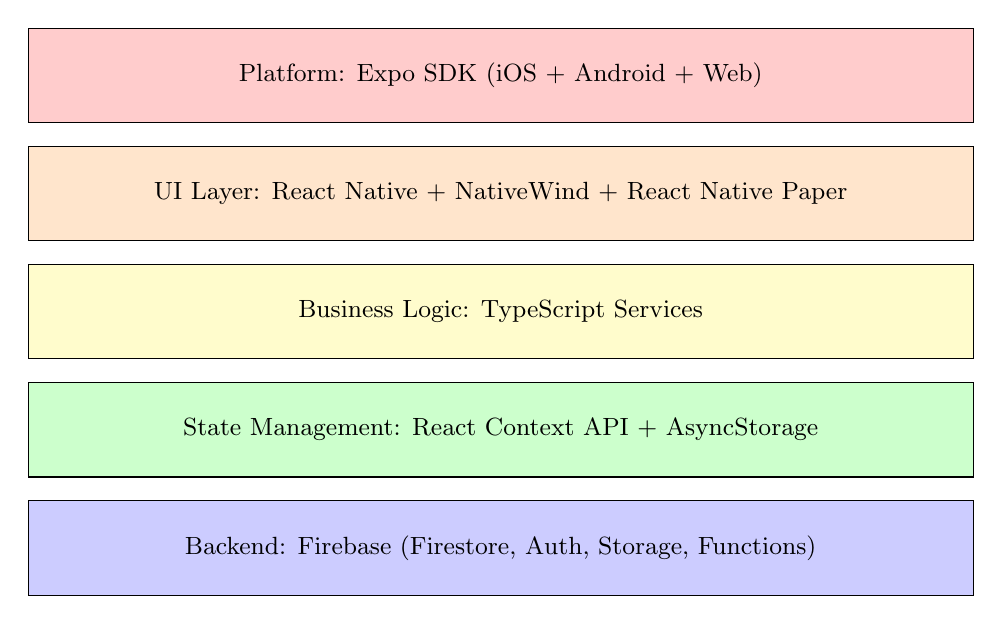
\begin{tikzpicture}[
    layer/.style={rectangle, draw, minimum width=12cm, minimum height=1.2cm, align=center, font=\small},
    arrow/.style={->, thick}
]
% Layers from bottom to top
\node[layer, fill=blue!20] (backend) at (0,0) {Backend: Firebase (Firestore, Auth, Storage, Functions)};
\node[layer, fill=green!20] (state) at (0,1.5) {State Management: React Context API + AsyncStorage};
\node[layer, fill=yellow!20] (logic) at (0,3) {Business Logic: TypeScript Services};
\node[layer, fill=orange!20] (ui) at (0,4.5) {UI Layer: React Native + NativeWind + React Native Paper};
\node[layer, fill=red!20] (platform) at (0,6) {Platform: Expo SDK (iOS + Android + Web)};
\end{tikzpicture}
\caption{Технологийн стекийн архитектур}
\label{fig:tech-stack}
\end{figure}

\textbf{Давхаргуудын тайлбар:}

\begin{itemize}
    \item \textbf{Platform Layer (Платформын давхарга):} Expo SDK нь iOS, Android, Web гурван платформд нэг кодоор ажиллах боломжийг олгоно. Expo-ийн бэлэн модулиуд (Camera, Location, Notifications) нь native код бичихгүйгээр төхөөрөмжийн боломжуудад хандана.
    
    \item \textbf{UI Layer (Хэрэглэгчийн интерфэйсийн давхарга):} React Native компонентууд, React Native Paper (Material Design), NativeWind (TailwindCSS) хамтран ажиллаж гоёмсог, responsive UI үүсгэнэ. Reanimated болон Gesture Handler нь анимаци, жестүүдийг удирдана.
    
    \item \textbf{Business Logic Layer (Бизнес логикийн давхарга):} TypeScript-ээр бичигдсэн service-үүд нь бизнес дүрмүүдийг хэрэгжүүлнэ. Жишээ нь: захиалгын тооцоо, хүргэлтийн төлөв шинэчлэлт, мэдэгдэл илгээх логик.
    
    \item \textbf{State Management Layer (Төлөв удирдлагын давхарга):} React Context API нь global state (хэрэглэгчийн мэдээлэл, сагс, тохиргоо) удирдана. AsyncStorage нь offline горимд өгөгдөл хадгална.
    
    \item \textbf{Backend Layer (Backend давхарга):} Firebase үйлчилгээнүүд (Firestore, Authentication, Storage, Cloud Functions) нь серверийн бүх функцийг хариуцна. Real-time синхрончлол, offline support, аюулгүй байдал бүгд Firebase-аар хангагдана.
\end{itemize}

\textbf{Өгөгдлийн урсгал (Data Flow):}

\begin{enumerate}
    \item Хэрэглэгч UI дээр үйлдэл хийнэ (товч дарах, form бөглөх)
    \item UI компонент event handler-ийг дуудна
    \item Handler нь Context-ийн функцийг дуудна
    \item Context нь Firebase SDK-аар серверт хүсэлт илгээнэ
    \item Firebase өгөгдлийг боловсруулж, хариу буцаана
    \item Context state-ийг шинэчилнэ
    \item React компонентуудыг дахин render хийнэ
    \item UI шинэчлэгдэнэ
\end{enumerate}

\textbf{Технологийн нэгтгэлийн үр дүн:}

\begin{table}[H]
\centering
\caption{Технологийн нэгтгэлийн үр дүн}
\label{tab:tech-benefits}
\begin{tabular}{|l|p{10cm}|}
\hline
\textbf{Үзүүлэлт} & \textbf{Үр дүн} \\
\hline
Хөгжүүлэлтийн хугацаа & Нэг платформд хөгжүүлэхтэй харьцуулахад 40-50\% бага \\
\hline
Кодын дахин ашиглалт & iOS, Android, Web хооронд 85-90\% код дахин ашиглагдсан \\
\hline
Гүйцэтгэл & 60 FPS, native аппликейшнтэй дүйцэхүйц \\
\hline
Offline support & Интернэтгүй үед ч үндсэн функцууд ажиллана \\
\hline
Real-time & Захиалгын төлөв өөрчлөгдөхөд 100ms дотор мэдэгдэл хүрнэ \\
\hline
\end{tabular}
\end{table}

\subsection{Ижил төстэй системүүдийн харьцуулалт}
Дэлхийн зах зээлд болон бүс нутгийн хэмжээнд ашиглагдаж буй ижил төстэй системүүдийг харьцуулан судлав.

\begin{longtable}{|p{2.5cm}|p{3.5cm}|p{3.5cm}|p{3.5cm}|}
\caption{Ижил төстэй системүүдийн харьцуулалт} \label{tab:comparison} \\
\hline
\textbf{Шалгуур} & \textbf{Lalamove (Ази)} & \textbf{Borzo (ОХУ/Монгол)} & \textbf{Tdelivery (Санал болгож буй)} \\
\hline
\endfirsthead
\hline
\textbf{Шалгуур} & \textbf{Lalamove (Ази)} & \textbf{Borzo (ОХУ/Монгол)} & \textbf{Tdelivery (Санал болгож буй)} \\
\hline
\endhead
\hline
\endfoot
\hline
\endlastfoot

\textbf{Үндсэн зорилго} & C2C, B2C Шуурхай хүргэлт & Crowdsourced хүргэлт & B2B Бараа түгээлт, SCM \\
\hline
\textbf{Хэрэглэгчид} & Хувь хүн, Жижиг бизнес & Хувь хүн, Онлайн дэлгүүр & Бөөний төв, Дэлгүүр, Нийлүүлэгч \\
\hline
\textbf{Тээврийн хэрэгсэл} & Мотоцикл, Ван, Машин & Явган, Мото, Машин & Портер, Ван (Ачаа тээвэр) \\
\hline
\textbf{Real-time Tracking} & Маш сайн & Сайн & Сайн \\
\hline
\textbf{Маршрут оновчлол} & AI суурьтай, автомат хуваарилалт & Автомат хуваарилалт & Google Maps API, Гараар болон автомат \\
\hline
\textbf{Төлбөрийн шийдэл} & Онлайн, Бэлэн & Бэлэн, Данс, COD & Бэлэн, Данс, Зээл (Credit) \\
\hline
\textbf{e-POD} & Зураг, Гарын үсэг & Зураг & Зураг, Гарын үсэг, GPS \\
\hline
\textbf{Үнэ} & Зайнаас хамаарсан & Зайнаас хамаарсан & Захиалгын дүнгийн хувь, эсвэл сарын хураамж \\
\hline
\textbf{Сул тал} & B2B нарийн процесс (нэхэмжлэх, буцаалт) дутмаг & Тогтмол хүргэгчгүй, найдвартай байдал сул & Зах зээлд шинэ, хэрэглэгчийн бааз бага \\
\hline
\end{longtable}

\subsubsection{Харьцуулсан дүгнэлт}
Lalamove болон Borzo нь "On-demand" буюу яаралтай, нэг удаагийн хүргэлтэд маш сайн шийдэл боловч B2B харилцааны нарийн процессуудыг (бараа буцаалт, зээлийн тооцоо, тогтмол маршрут, их хэмжээний бараа хүлээлцэх) бүрэн шийдэж чадахгүй байна. "Tdelivery" систем нь эдгээр дутагдлыг нөхөж, Монголын жижиг дунд бизнесүүдийн онцлогт тохирсон, нийлүүлэлтийн сүлжээг бүхэлд нь хамарсан шийдэл болохоороо давуу талтай юм.

\vfill